\documentclass{ENZCon}

\usepackage{graphicx} 

\begin{document}

\title{Debugging Grounding and EMI Problems in Development of an Autonomous Go-kart}

\author{Nissanka Weerekoon\\
Email: naw52@uclive.ac.nz \\
$Supervisor:$ Dr Andrew Bainbridge-Smith\\
andrew.bainbridge-smith@canterbury.ac.nz\\
\\
Department of Mechatronics Engineering\\
University of Canterbury, New Zealand}

\abstract{This paper proposes methods to debug grounding and electromagnetic interference problems during the development of an autonomous go-kart. Good hardware debugging practises were explored and used to generate two procedures. These successfully isolated and verified the hypothesized causes. The go-kart control system design first began in 2011 and this paper only focuses on a small portion of the work done this year, as part of a final year project. Debugging of these problems, along with others, allowed basic movement control of the go-kart and integration with computer vision navigation to be successfully demonstrated.
}

\keywords{Autonomous, Grounding, Electromagnetic Interference, Go-kart, Drive-by-wire, CANBus}

\maketitle

\section{Introduction}

Development of an autonomous vehicle is a large task, drawing from many areas of engineering knowledge. For this reason the University of Canterbury Autonomous Go-kart Project was divided such that individuals and teams would work on different aspects of development over multiple years, with an end goal towards developing a completely autonomous go-kart. The project as a whole was begun in 2011 and is designed around one of the Electrical Department's electric go-karts. In its first year, a team of four students began by choosing suitable actuators and designing five Controller Area Network bus (CANBus) printed circuit boards (PCBs)~\cite{Jenkins_2011, Looman_2011, Richards_2011, taylor_2011} . In 2012 a student developed an Application Programmer Interface (API) in Python to allow the CANBus system to be controlled via laptop commands ~\cite{Wigley_2012}. At the end of its second year, basic system communication and operation had been demonstrated on the laboratory bench, however it had never been mounted on the go-kart and no controlled movement of the go-kart had been achieved.

This year the project was undertaken by a single student and the portion toward the end goal to be completed 
consisted of two parts. The primary objective was to use the previously developed CANBus system to achieve basic movement control over the go-kart. The second part involved demonstrating proof of autonomous capability using computer vision navigation.

This paper focuses on the identification and solution to two issues encountered while attempting to mount the existing system on the go-kart. The state of the system prior to beginning work this year was such that steering and brake calibration routines along with unit tests could be successfully run on the system on the workbench. This meant that though the speed sensor was connected no speed reading could be taken. In addition no motor control or PWM generation could be demonstrated and all servo movement was unloaded. Due to a number of hardware faults in previous years and subsequent workarounds the hardware system was not at all robust. 

\subsection{System Overview}

The system developed thus far consists of five main PCBs that communicate with each other via a CANBus network as seen in Figure~\ref{fig:block}. Each board is responsible for controlling a particular aspect of go-kart movement which include: steering, brake, motor, speed sensing, and communications. The communications module allows control commands from a laptop via USB to be passed into the CANBus network and for requested values to be passed back to the laptop. This system what mounted on the go-kart for testing purposes as seen in Figure~\ref{fig:whole}. 

\begin{figure}[htbp]
	\centering
		\includegraphics[width=0.4\textwidth]{C:/Users/Nissanka/Desktop/Picture1.png}
	\caption{CANBus control system block diagram}
	\label{fig:block}
\end{figure}

The steering and brake PCBs interface with their respective actuators via a motor driver board. An encoder in each actuator sends a signal directly back to each PCB corresponding to positional movement. The speed sensor PCB reads an inductive proximity sensor mounted close to a sprocket on the rear axle. The motor control PCB interfaces with a pulse width modulation (PWM) generation board and motor driver electronics to power the go-kart's motor. It was designed in 2011 to send only the target motor duty cycle to the PWM generation board across a serial peripheral interface (SPI) connection. 

\begin{figure}[htbp]
	\centering
		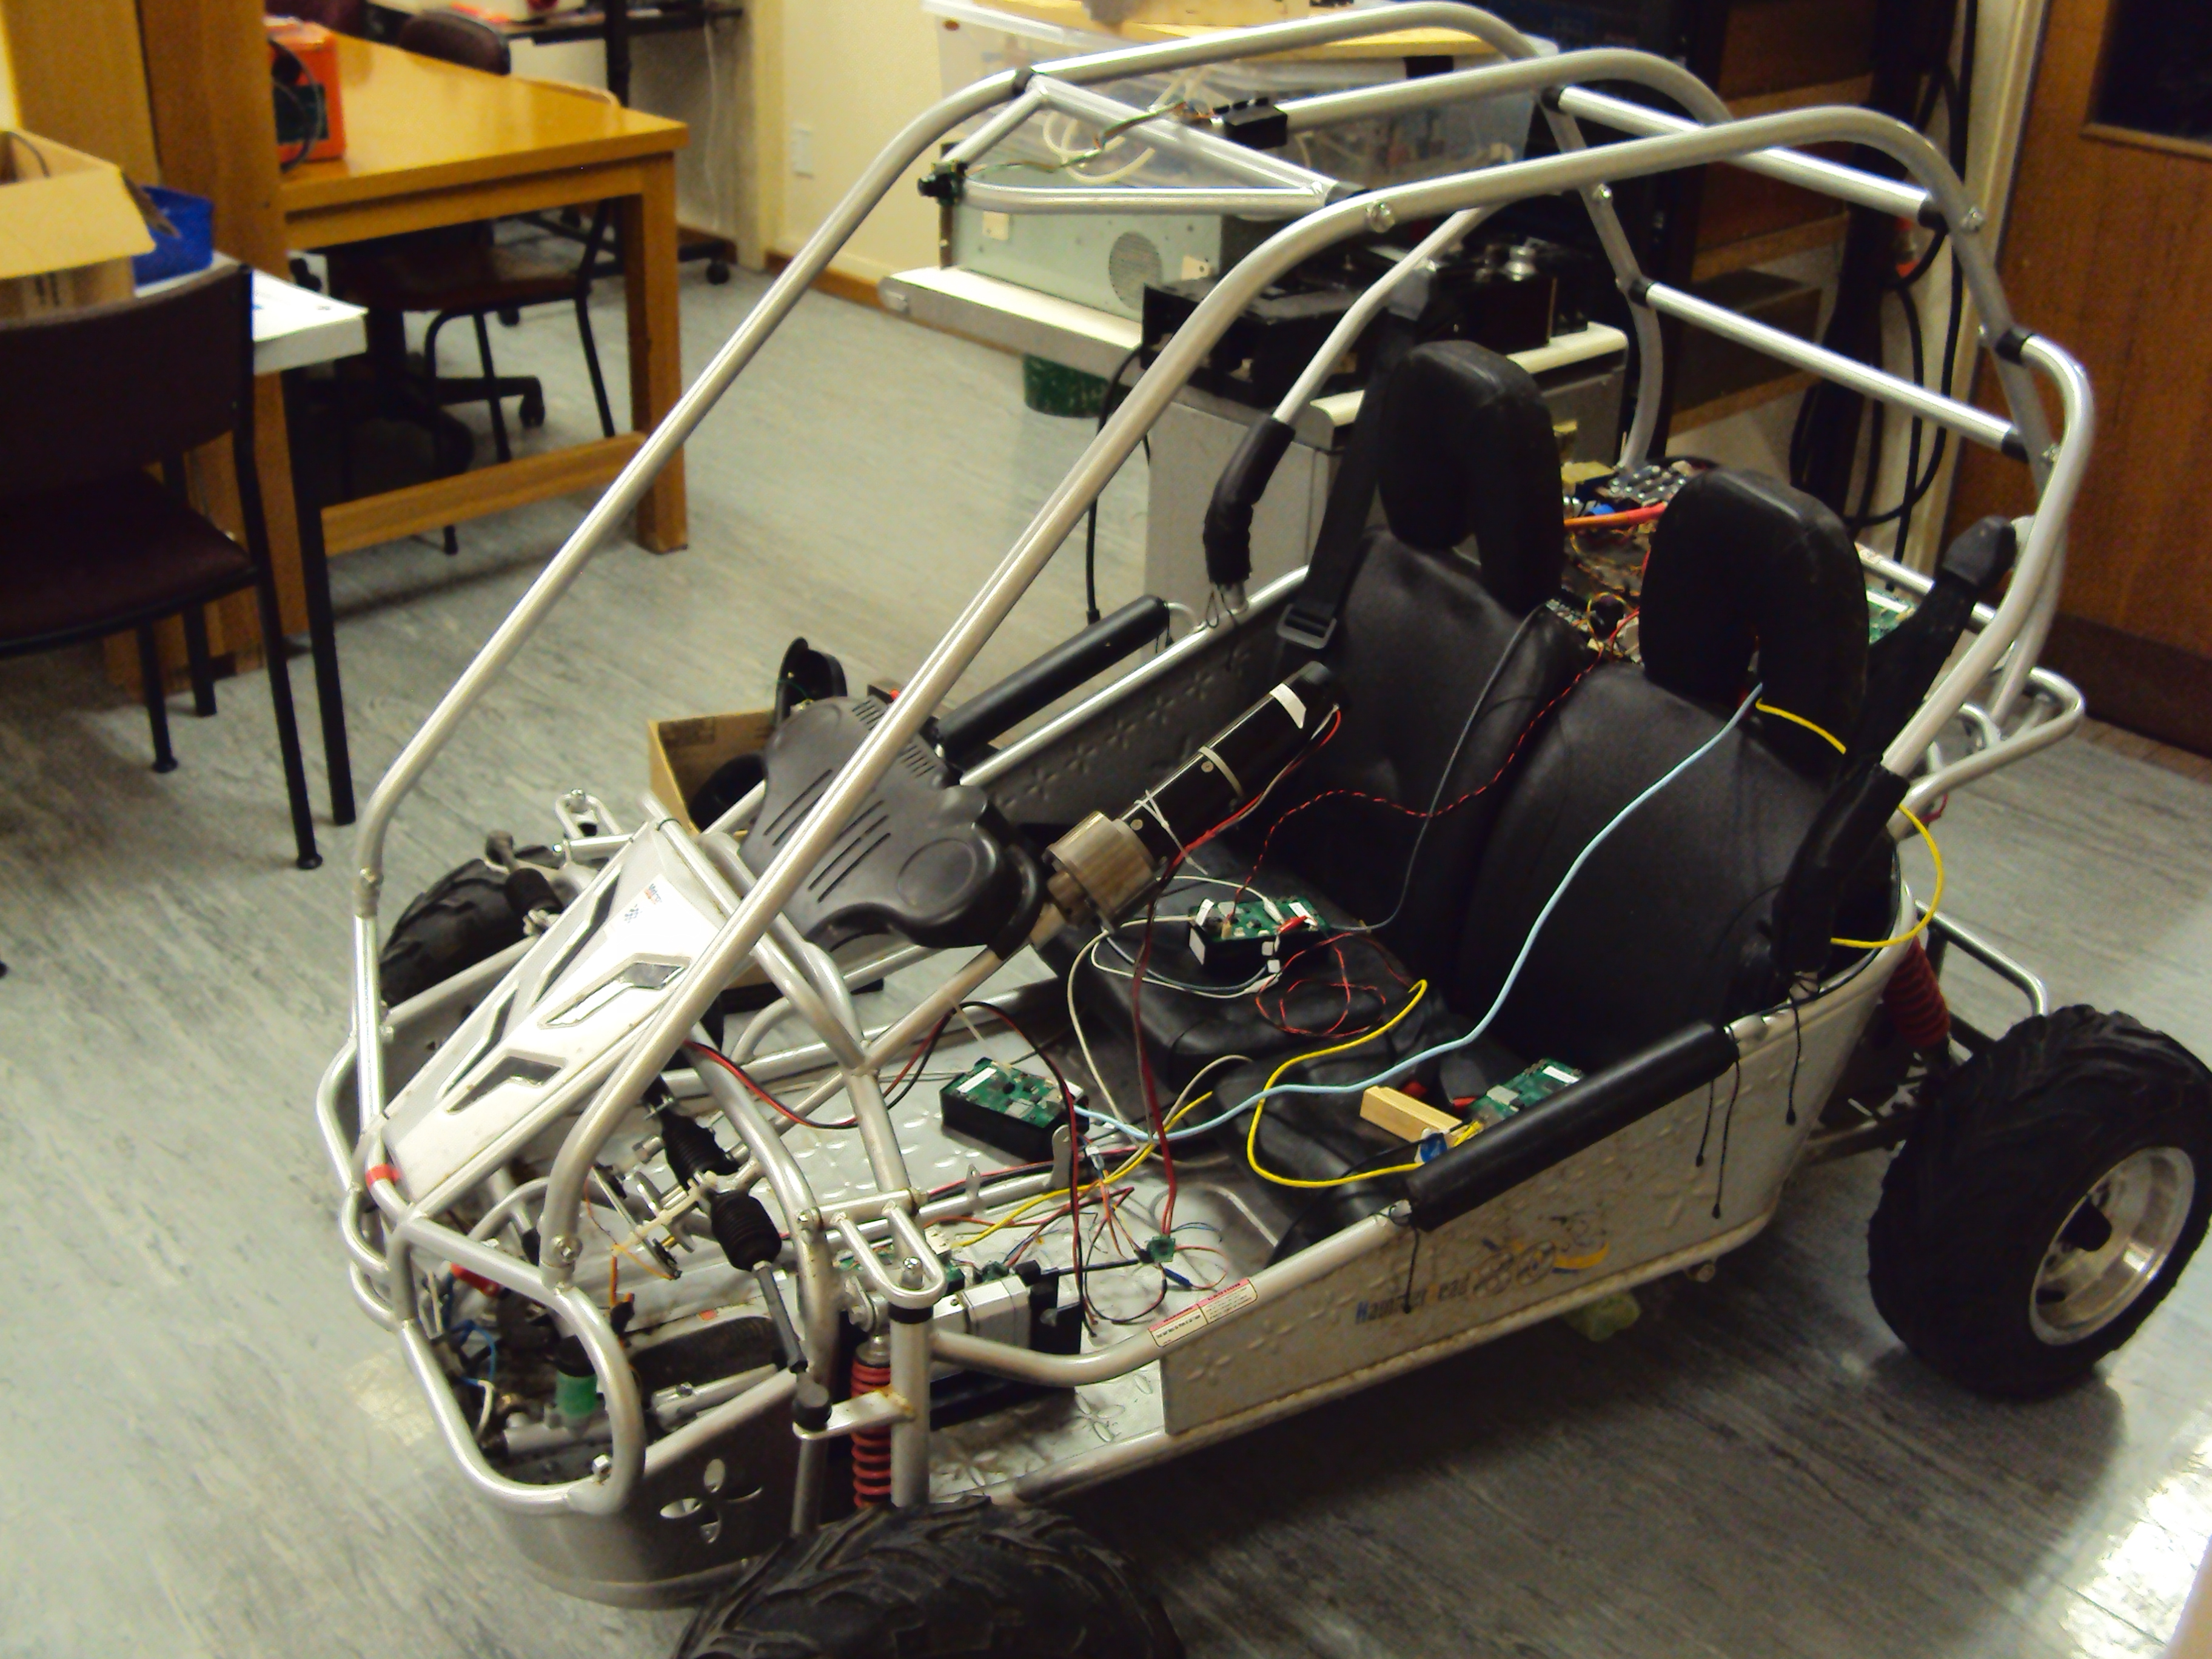
\includegraphics[width=0.40\textwidth]{C:/Users/Nissanka/Documents/Uni/3rd_pro/Project_Autonomous_Go_Kart/Mariokart2/Submissions/Research_paper/whole_2.JPG}
	\caption{CANBus control system on go-kart}
	\label{fig:whole}
\end{figure}

The control system and API had been designed such that upon power-up, the system would run through an initial calibration process independent of any laptop commands. If calibration routines completed successfully the system transitioned into a $Running$ state in which API commands could be used to control the steering, brake and motor independently from the laptop. An error or communication fault during any stage would cause the system to drop into an $Error$ state until power was recycled. 

\section{Debugging Theory}

\subsection{General debugging process}

In order to achieve successful and efficient testing and integration, Ball~\cite{ball_2002} recommends that a goal or plan should be clearly laid out in advance. He goes on to emphasise that embedded systems are difficult to debug as it can be unclear whether the problem lies in hardware or software and that sometimes hardware problems are best fixed in software and vice versa. This leads on to the interdependence problem of hardware and software in embedded systems; neither can always be fully tested independently. Foreseeing this problem, Ball suggests that writing software purely for the purposes of testing hardware may contribute more efficiently than testing hardware using software that itself is not fully tested and verified. Therefore when testing a previously untested hardware system there are two possible paths~\cite{ball_1998_debugging}:
\begin{enumerate}
	\item{Plug unproven code into hardware; start it up; observe.
Bugs tracked and dealt with one at a time
-Prone to leaving undetected errors in software}
	\item{Verify as far as possible with simple routines.
Get software framework that can exercise hardware.
Add and verify firmware functions one at a time.
-This is an idealized picture
-A point comes where path 1 must be taken.}
\end{enumerate}

To help facilitate this process with efficiency, Ball and many other debugging guides highly recommend keeping a logbook of symptoms and changes that have been made. This leads to focused debugging and a more systematic approach to isolating the bug. Symptoms should be highly detailed, especially any patterns or randomness observed. 

\subsection{Debugging Hardware Problems}

\subsubsection{Debugging grounding related problems}

The purpose of grounding an electrical system or microprocessor board is to provide it with a reference potential. Connecting a ground source ensures that any other point in the system stays at its given potential with reference to that ground~\cite{grounding_practical}. In the case of vehicles, the negative terminal of the battery may be used as the ground reference and connected to the chassis~\cite{patent}. This highlights the fact that a voltage sensed by a device is only relative to its reference, therefore ground references used across the entire system should have the same potential.

In~\cite{ball_1998_debugging} Ball lists a number of possible grounding related issues, mainly involving floating pins. Many CMOS parts are said to work without a ground connection as long as one of the inputs is low, but when they all transition to a high state everything appears to stop. 

\subsubsection{Debugging EMI related problems}

Inductive devices such as the DC motor used on the electric go-kart are known to cause EMI when they are switched on and off. If wiring impedance is high enough the ground on the processor board can be upset far enough to affect operation or hinder communication with other boards in system. In~\cite{ball_1998_debugging} Ball says this is especially the case with PWM driven motors such as the go-kart motor. In the case of this project the motor is driven from separate drive circuitry rather than directly from the CANBus control boards. This, along with the CANBus data transfer method and use of four-layer PCBs should minimise noise and EMI issues. However noise may still be passed through interconnected grounds. 

Connectors and cables joining various parts of an electrical system can be highly susceptible to EMI especially if they are uninsulated. As explained in~\cite{grounding_practical} EMI suppression can be achieved by using metallic conduit as a grounding conductor because it acts as a screen for electromagnetic flux. This protects the signals within the conduit, similar to shielding. 

\section{Problem Solving}

\subsection{Grounding fault isolation}

One of the first hurdles encountered while trying to get the existing system running on the go-kart was incomplete calibration. In particular, steering calibration involved panning the full range of steering motion, touching limit switches at the base of the steering column at either end of this range. Software on the steering PCB used the steering servo encoder signals to log a positional value for each extreme and calculate the centre steering position. The system would turn the wheels all the way in one direction, until the limit switch was triggered. From here however the steering servo would stop turning when it was meant to turn in the reverse direction to trigger the other limit switch. 

As a first step, a log for this bug was created and the nature of the symptoms such as any randomness and the current system configuration including all connections were documented. This provided a reference point for comparison when changes and fixes were attempted.

The go-kart's power supply and motor driver electronics were undergoing a reconfiguration process separate to this project. Therefore the actuators and CANBus boards were powered using separate 24V DC bench supplies, similar to the bench testing setup.Therefore the only differences to the bench testing setup were the actuator moving under load and the system being placed around the go-kart rather than on bench. 

The next series of steps were conducted to eliminate potential factors affecting the problem and isolate its cause. The results of each test or process were recorded to ensure a focused thorough process. 


\begin{table}[tbp]
	\centering
		\begin{tabular}{|p{0.22\textwidth}|p{0.22\textwidth}|}
		\hline
		\textbf{Process} & \textbf{Results}\\
		\hline
		Changes in configuration between go-kart and bench setup investigated and eliminated - used different bench power supplies, reduced actuator load. & Cycling only the actuator power supply when the problem occurred caused calibration to resume and complete fully. This hinted to a problem with the motor driver board but it was important to maintain a systematic isolation process and not jump to conclusions.\\
		\hline
		Probing the signals from the steering PCB to its motor driver board it was evident that these PWM signals ($IN1$ and $IN2$ in Figure~\ref{fig:Sch}) changed correctly. & This suggested a hardware problem, especially since no software changes had been made to calibration since porting the system from bench.\\
		\hline
		Entire system checked for loose/incorrect connections. & Eliminated problem with existing hardware connections. Problem is isolated to effect on hardware due to on-kart environment.\\
		\hline
		Motor driver board and steering actuator datasheets checked for possible causes. & As seen in~\ref{fig:Sch} the motor driver has separate power ground (PGND) and analog ground (AGND) connections. AGND had no connection directly to ground on the steering board.\\
		\hline			
		\end{tabular}
	\caption{Grounding Issue: Elimination and Isolation Process}
	\label{tab:grounding}
\end{table}

\begin{figure}[h!]
	\centering
		\includegraphics[width=0.35\textwidth]{C:/Users/Nissanka/Desktop/Capture.JPG}
	\caption{Motor driver connection schematic}
	\label{fig:Sch}
\end{figure}


The systematic process undertaken in Table ~\ref{tab:grounding} revealed that as per the schematic only $EN$, $IN1$ and $IN2$ were connected between the steering PCB and its motor driver board. As there was no ground connection directly between the two boards, the ground reference was only shared back through the power supplies connecting the actuators and the CANBus boards. From the perspective of the motor driver board, the signals coming from the steering PCB were with respect to the high power ground line used to drive the steering actuator.



\subsection{EMI problem isolation}

Due to the motor electronics not being ready for testing CANBus motor control on the delegated go-kart, the motor controlability was tested separately on another go-kart. As there were no actuator attachments on this other go-kart, the CANBus system was reduced to connect only the motor, speed sensor and communication nodes for simplicity. Motor control was then successfully implemented, requiring only the target duty cycle or speed to be sent from the laptop via the API. For verifying basic movement control, only duty cycle control was used to isolate any problems to the motor module. 


When the complete system was finally able to be set up on one go-kart, it was observed that steering control was lost soon after the motor made to run. Similar to the previous grounding bug, a systematic process of logging symptoms, fixes and responses was begun. Again it was unsure if the problem was related to software, hardware or both as neither had been individually verified under these conditions. 

The problem was such that when all five CANBus PCBs were connected and the motor was run, the steering board character display lost one digit, the steering became unresponsive and the system transitioned into an error state. A fault in the steering board only when the motor was run was speculated to be an EMI related issue and a isolation via elimination process was devised and carried out to verify this, as outlined in Table~\ref{tab:EMI}.



The debugging process carried out found that the connection from the steering PCB to the steering calibration limit switches was inducing a large disturbance in the steering board electronics when the motor was running, enough to put it into an unresponsive state.


\section{Testing and Results}

Making a ground connection directly between the steering control PCB and the steering motor drive board allowed calibration to proceed successfully. The motor driver board gets a direct ground reference from the steering PCB for more accurate comparisons and the control and high power signals are maintained separately. 

In terms of the limit switch connection, replacing the previously used ribbon cable with various types of shielded wire had no effect. However, when nylon nuts and bolts instead of steel were used to fasten the limit switch locating plate to the chassis as seen in Figure~\ref{fig:lim_sw}, the problem was solved and the motor and steering could be controlled independently. This suggests the chassis and limit switch cable combination having and antennae effect, causing motor EMI to effect only the steering board. This was also verified when a Tesla coil was by chance operated in the vicinity of the go-kart, causing the steering board to be effected significantly worse than any other board. 



\begin{table}[htbp]
	\centering
		\begin{tabular}{|p{0.22\textwidth}|p{0.22\textwidth}|}
		\hline
		\textbf{Process} & \textbf{Results}\\
		\hline
		Attempted to simply isolate involved hardware modules by running system leaving out one CANBus module at a time. & System functioned correctly when steering board disconnected.\\
		\hline
		Error state transition = bug triggering code response. Therefore used character display to identify point at which each board moves to error state & Communications board found to be pinging all boards. Failed response from steering board triggered timeout into Error state.\\
		\hline
		Communications reduction: messages only passed from python API via communications board to motor board & Problem not caused by API communication to steering board\\
		\hline
		Further communications reduction: removed CANBus network ping from communications board to motor board and error state transition commands. Calibration handshaking still required to control steering & Steering board in idle state with no communications to/from it but display loses one digit - not software controlled.\\
		\hline			
		Systematically remove hardware connections steering board after calibration except CANBus/power & Disconnecting steering limit switch cable after calibration allows steering to be controlled while motor running.\\
		\hline
		\end{tabular}
	\caption{EMI Issue: Elimination and Isolation Process}
	\label{tab:EMI}
\end{table}

\begin{figure}[htbp]
	\centering
		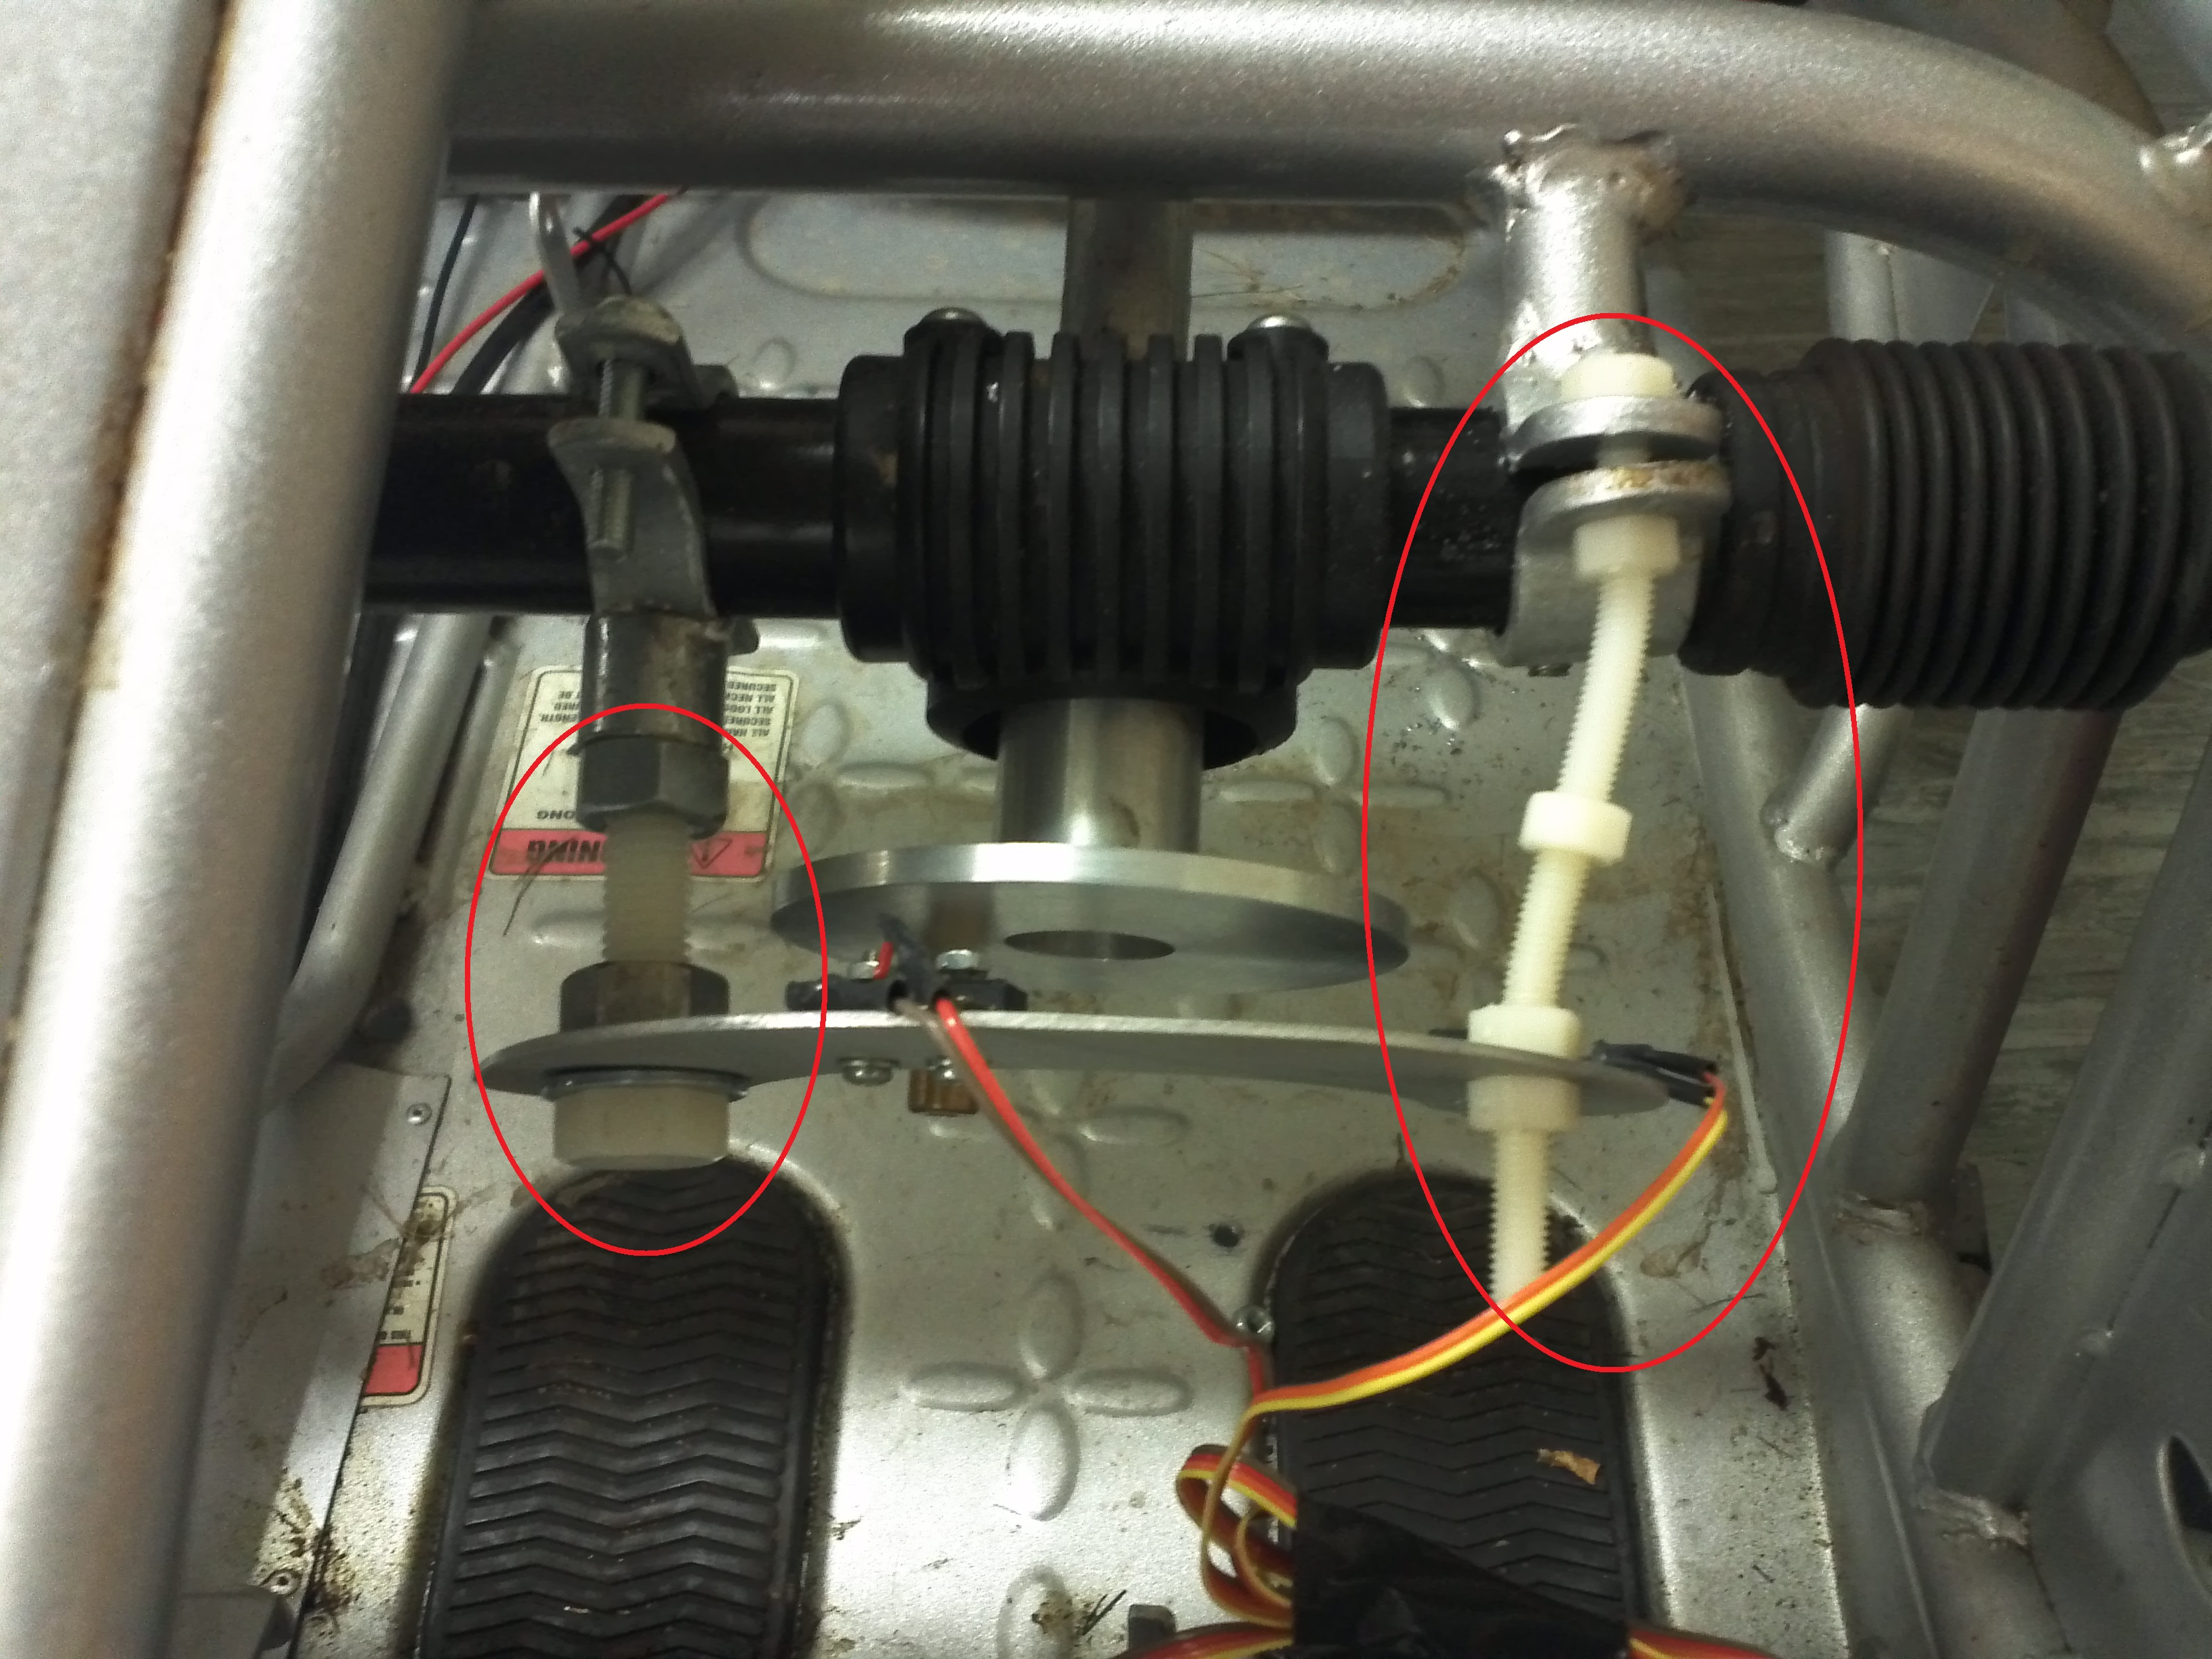
\includegraphics[width=0.40\textwidth]{C:/Users/Nissanka/Documents/Uni/3rd_pro/Project_Autonomous_Go_Kart/Mariokart2/Submissions/Research_paper/lim_sw.jpg}
	\caption{Modified Limit Switch Attachment}
	\label{fig:lim_sw}
\end{figure}




\section{Conclusion}

The debugging methods outlined in this paper enabled project development to continue this year and be successful in achieving the goals set. Two problems in an existing multi-processor embedded system were identified when the system was moved on to the go-kart. These were incorrect grounding between boards and EMI, which were not testable or identifiable during the previous bench testing. A systematic debugging approach was constructed based on standard industry practises and followed to isolate, verify and eliminate the problems. 

This progress was only one portion of the work done towards the autonomous go-kart project this year. Once these problems along with other challenges were overcome, the entire CANBus system was successfully mounted on the go-kart. A graphical user interface (GUI) was developed along side this process to easily allow testing and basic control over each of the go-kart's modules by developers. In addition, a computer vision based checkerboard tracking algorithm written in C++ was interfaced to the Python API. The second portion of this year's goals was then completed by making the go-kart autonomously track the checkerboard, while maintaining a set distance from it. 

This work done on the project creates two possible paths for future work. The first would be to research and develop a better autonomous navigation system using computer vision and/or other sensors connected to the CANBus sensor board. This development should use the existing CANBus control hardware to develop the system. The second path involves renewing the current CANBus control hardware to ensure the go-kart is robust and fit for field testing. The fabrication of at least five new CANBus PCBs with more robust connectors is recommended as a starting point. It is also emphasised that both these paths can and should be conducted simultaneously to make maximum progress towards an autonomous go-kart in the given time. 

% DO NOT USE a bibliographystyle{} -- it is defined as ieeetr in the ENZCon class

\bibliography{go_kart}

\end{document}
